% =====================================================================
%  ncwu_calc_notes_color
%  来源：高等数学课堂笔记（彩色多变主题）（YangTex 模板库 · 用户原稿全量保留版）
%  处理：仅删除编译产物 PDF / digest.lock，把 \input 递归展开为单文件；
%        正文、章节、例题、每张幻灯片、封面与参考文献一字未改。
%  字体：原稿的 macOS 字体声明全部保留，外加 \IfFontExistsTF 存在性判断；
%        在 Mac 上视觉与原 PDF 完全一致，在 Windows / Linux 上字体缺失时
%        自动跳过该声明改用默认字体，仍能正常编译。
%  编译：xelatex（目录 / 交叉引用需连续编译 2~3 遍，产品已自动处理）
% =====================================================================

% !TEX program = xelatex
% =====================================================================
%  高等数学课堂笔记 —— 格式精美 · 色彩多变 · 个性张扬
%  作者：杨建伟（华北水利水电大学 数学与统计学院）
%  编译：xelatex -> xelatex （运行两遍以生成目录）
% =====================================================================
\documentclass[11pt,a4paper]{article}

% ---------- 中文支持 ----------
\usepackage{ctex}
\usepackage{fontspec}

% ---------- 颜色 / 几何 / 盒子 ----------
\usepackage{xcolor}
\usepackage[most]{tcolorbox}
\usepackage{tikz}
\usepackage{pgfplots}
\pgfplotsset{compat=1.18}
\usetikzlibrary{shadows,positioning,decorations.pathmorphing,arrows.meta,calc,patterns,shapes.callouts,shapes.geometric}

% ---------- 数学 ----------
\usepackage{amsmath,amssymb,amsthm,mathtools}
\usepackage{unicode-math}  % 仅在 XeLaTeX 下

% ---------- 排版辅助 ----------
\usepackage{geometry}
\geometry{left=2.2cm,right=2.2cm,top=2.4cm,bottom=2.2cm,headheight=15pt,footskip=1.2cm}
\usepackage{fancyhdr}
\usepackage{titlesec}
\usepackage{titletoc}
\usepackage{enumitem}
\usepackage{multicol}
\usepackage{dashrule}
\usepackage{pagecolor}
\usepackage{eso-pic}
\usepackage{hyperref}

% ---------- 自定义糖果色板 ----------
% ============================================================
%  炫彩色板 —— 更饱和 · 更靓丽 · 更有层次
% ============================================================
% --- 主色（更饱和更亮） ---
\definecolor{cBlue}{HTML}{1565C0}      % 明亮宝蓝
\definecolor{cBlueL}{HTML}{E3F2FD}     % 冰蓝底
\definecolor{cBlueLL}{HTML}{BBDEFB}    % 中间蓝
\definecolor{cPink}{HTML}{D81B60}      % 鲜艳玫红
\definecolor{cPinkL}{HTML}{FCE4EC}
\definecolor{cPurple}{HTML}{8E24AA}    % 亮紫
\definecolor{cPurpleL}{HTML}{F3E5F5}
\definecolor{cTeal}{HTML}{00838F}      % 翠青
\definecolor{cTealL}{HTML}{E0F7FA}
\definecolor{cOrange}{HTML}{E64A19}    % 烈焰橙
\definecolor{cOrangeL}{HTML}{FBE9E7}
\definecolor{cYellow}{HTML}{FFA000}    % 金黄
\definecolor{cYellowL}{HTML}{FFF8E1}
\definecolor{cGreen}{HTML}{2E7D32}     % 翠绿
\definecolor{cGreenL}{HTML}{E8F5E9}
\definecolor{cInk}{HTML}{1A1A2E}       % 深墨
\definecolor{cIndigo}{HTML}{4527A0}    % 深靛蓝
\definecolor{cIndigoL}{HTML}{EDE7F6}   % 淡靛蓝
\definecolor{cPaper}{HTML}{FAFAFF}     % 纸色
% --- 霓虹强调色 ---
\definecolor{nCyan}{HTML}{00E5FF}
\definecolor{nMagenta}{HTML}{FF1744}
\definecolor{nGold}{HTML}{FFD600}
\definecolor{nPurple}{HTML}{D500F9}
\definecolor{nOrange}{HTML}{FF6D00}
\definecolor{nLime}{HTML}{76FF03}

\pagecolor{cPaper}
\color{cInk}


% ---------- 超链接颜色 ----------
\hypersetup{colorlinks=true,linkcolor=cBlue,urlcolor=cPurple,citecolor=cTeal}
% ============================================================
%  炫酷页眉页脚 —— 渐变色条 + 彩色圆点
% ============================================================
\pagestyle{fancy}
\fancyhf{}
\renewcommand{\headrulewidth}{0pt}
\renewcommand{\footrulewidth}{0pt}

% 渐变页眉色条
\renewcommand{\headrule}{%
  \vspace{-2pt}%
  \tikz{%
    \shade[left color=cBlue, right color=cPurple]
      (0,0) rectangle (\linewidth, 2.5pt);%
    \fill[cBlue]      (0.03*\linewidth, 1.25pt) circle (2pt);%
    \fill[cPink]      (0.25*\linewidth, 1.25pt) circle (1.5pt);%
    \fill[cYellow]    (0.50*\linewidth, 1.25pt) circle (1.5pt);%
    \fill[cTeal]      (0.75*\linewidth, 1.25pt) circle (1.5pt);%
    \fill[cPurple]    (0.97*\linewidth, 1.25pt) circle (2pt);%
  }%
  \vspace{-4pt}%
}

\fancyhead[L]{%
  \tikz[baseline=-0.5ex]{
    \fill[cBlue] (0,0) circle (3pt);
    \fill[cPink] (0.45,0) circle (2pt);
  }%
  \;\small\sffamily\bfseries\color{cBlue}高等数学课堂笔记%
}
\fancyhead[R]{%
  \small\sffamily\bfseries\color{cPurple}杨建伟%
  \;\tikz[baseline=-0.5ex]{
    \fill[cPurple] (0,0) circle (3pt);
    \fill[cTeal] (0.45,0) circle (2pt);
  }%
}


\fancyfoot[C]{%
  
\begin{tikzpicture}
    \node[fill=cBlue, text=white, circle, inner sep=2pt, minimum size=24pt, font=\small\bfseries]
      {\thepage};
  \end{tikzpicture}}
\fancyfoot[L]{\small\color{gray}华北水利水电大学 · 数学与统计学院}
\fancyfoot[R]{\small\color{gray}\rightmark}

% ---------- 章节标题样式 ----------
\titleformat{\section}
  {\sffamily\bfseries\LARGE\color{cBlue}}
  {\tikz[baseline=-0.6ex]\node[fill=cPink, text=white, rounded corners=6pt, inner xsep=10pt, inner ysep=3pt, font=\bfseries\large]{\thesection};}
  {0.7em}
  {\color{cBlue}}
  [\vspace{3pt}{\color{cBlue!50}\titlerule[1.5pt]}]

\titleformat{\subsection}
  {\sffamily\bfseries\large\color{cPurple}}
  {\tikz[baseline=-0.5ex]\node[fill=cYellow, text=cInk, rounded corners=5pt, inner xsep=8pt, inner ysep=2.5pt, font=\bfseries]{\thesubsection};}
  {0.55em}{}

% ---------- 目录样式优化 ----------
\titlecontents{section}
  [0pt]
  {\addvspace{8pt}\sffamily\bfseries\normalsize}
  {\tikz[baseline=-0.55ex]\node[fill=cBlue, text=white, rounded corners=4pt,
     inner xsep=6pt, inner ysep=2pt, font=\normalsize\bfseries]{\thecontentslabel};\hspace{0.7em}}
  {}
  {\;\color{gray!60}\titlerule*[6pt]{.}\;\contentspage}

\titlecontents{subsection}
  [1.6cm]
  {\addvspace{3pt}\sffamily\small}
  {\textcolor{cPurple}{\thecontentslabel}\hspace{0.5em}}
  {\color{cInk}}
  {\;\color{gray!60}\titlerule*[6pt]{.}\;\contentspage}

% ---------- 通用 tcolorbox 样式：贴纸质感 + 靓丽渐变底 ----------
% 基础样式提取到 tcbset，减少重复；编号版与无编号版共用同一 base
\tcbset{
  defbase/.style={
    enhanced, breakable,
    arc=12pt, outer arc=14pt,
    drop fuzzy shadow=gray!40,
    fonttitle=\sffamily\bfseries,
    coltitle=white,
    title style={left color=cBlue, right color=cBlue!75!black},
    boxrule=1.2pt, colframe=cBlue!50,
    interior style={top color=cBlue!40, bottom color=cBlue!12},
    attach boxed title to top left={xshift=8pt, yshift=-7pt},
    boxed title style={arc=8pt, boxrule=0pt, top=3pt, bottom=3pt, left=8pt, right=8pt},
    top=14pt, bottom=8pt, left=10pt, right=10pt,
    before skip=12pt, after skip=10pt,
  },
  thmbase/.style={
    enhanced, breakable,
    arc=12pt, outer arc=14pt,
    drop fuzzy shadow=gray!40,
    fonttitle=\sffamily\bfseries,
    coltitle=white,
    title style={left color=cPurple, right color=cPurple!75!black},
    boxrule=1.2pt, colframe=cPurple!50,
    interior style={top color=cPurple!38, bottom color=cPurple!10},
    attach boxed title to top left={xshift=8pt, yshift=-7pt},
    boxed title style={arc=8pt, boxrule=0pt, top=3pt, bottom=3pt, left=8pt, right=8pt},
    top=14pt, bottom=8pt, left=10pt, right=10pt,
    before skip=12pt, after skip=10pt,
  },
  egbase/.style={
    enhanced, breakable,
    arc=12pt, outer arc=14pt,
    drop fuzzy shadow=gray!40,
    fonttitle=\sffamily\bfseries,
    coltitle=white,
    title style={left color=cTeal, right color=cTeal!75!black},
    boxrule=1.2pt, colframe=cTeal!50,
    interior style={top color=cTeal!38, bottom color=cTeal!10},
    attach boxed title to top left={xshift=8pt, yshift=-7pt},
    boxed title style={arc=8pt, boxrule=0pt, top=3pt, bottom=3pt, left=8pt, right=8pt},
    top=14pt, bottom=8pt, left=10pt, right=10pt,
    before skip=12pt, after skip=10pt,
  },
  tipbase/.style={
    enhanced, breakable,
    arc=12pt, outer arc=14pt,
    drop fuzzy shadow=gray!40,
    fonttitle=\sffamily\bfseries,
    coltitle=white,
    title style={left color=cOrange, right color=cOrange!75!black},
    boxrule=1.2pt, colframe=cOrange!50,
    interior style={top color=cOrange!35, bottom color=cOrange!10},
    attach boxed title to top left={xshift=8pt, yshift=-7pt},
    boxed title style={arc=8pt, boxrule=0pt, top=3pt, bottom=3pt, left=8pt, right=8pt},
    top=14pt, bottom=8pt, left=10pt, right=10pt,
    before skip=12pt, after skip=10pt,
  },
  warnbase/.style={
    enhanced, breakable,
    arc=12pt, outer arc=14pt,
    drop fuzzy shadow=gray!40,
    fonttitle=\sffamily\bfseries,
    coltitle=white,
    title style={left color=cPink, right color=cPink!75!black},
    boxrule=1.2pt, colframe=cPink!50,
    interior style={top color=cPink!35, bottom color=cPink!10},
    attach boxed title to top left={xshift=8pt, yshift=-7pt},
    boxed title style={arc=8pt, boxrule=0pt, top=3pt, bottom=3pt, left=8pt, right=8pt},
    top=14pt, bottom=8pt, left=10pt, right=10pt,
    before skip=12pt, after skip=10pt,
  },
  sumbase/.style={
    enhanced, breakable,
    arc=12pt, outer arc=14pt,
    drop fuzzy shadow=gray!40,
    fonttitle=\sffamily\bfseries,
    coltitle=white,
    title style={left color=cGreen, right color=cGreen!75!black},
    boxrule=1.2pt, colframe=cGreen!50,
    interior style={top color=cGreen!35, bottom color=cGreen!10},
    attach boxed title to top left={xshift=8pt, yshift=-7pt},
    boxed title style={arc=8pt, boxrule=0pt, top=3pt, bottom=3pt, left=8pt, right=8pt},
    top=14pt, bottom=8pt, left=10pt, right=10pt,
    before skip=12pt, after skip=10pt,
  },
  eggbase/.style={
    enhanced, breakable,
    arc=12pt, outer arc=14pt,
    drop fuzzy shadow=gray!40,
    fonttitle=\sffamily\bfseries,
    coltitle=cInk,
    title style={left color=cYellow, right color=cOrange!80},
    boxrule=1.2pt, colframe=cYellow!60,
    interior style={top color=cYellow!45, bottom color=cYellow!12},
    attach boxed title to top left={xshift=8pt, yshift=-7pt},
    boxed title style={arc=8pt, boxrule=0pt, top=3pt, bottom=3pt, left=8pt, right=8pt},
    top=14pt, bottom=8pt, left=10pt, right=10pt,
    before skip=12pt, after skip=10pt,
  },
  plainbase/.style={
    enhanced, breakable,
    arc=12pt, outer arc=14pt,
    drop fuzzy shadow=gray!40,
    fonttitle=\sffamily\bfseries,
    coltitle=white,
    title style={left color=gray!60, right color=gray!45},
    boxrule=1.2pt, colframe=gray!40,
    interior style={top color=gray!22, bottom color=gray!8},
    attach boxed title to top left={xshift=8pt, yshift=-7pt},
    boxed title style={arc=8pt, boxrule=0pt, top=3pt, bottom=3pt, left=8pt, right=8pt},
    top=14pt, bottom=8pt, left=10pt, right=10pt,
    before skip=12pt, after skip=10pt,
  },
  proofbase/.style={
    enhanced, breakable,
    arc=12pt, outer arc=14pt,
    drop fuzzy shadow=gray!40,
    fonttitle=\sffamily\bfseries,
    coltitle=white,
    title style={left color=cIndigo, right color=cIndigo!75!black},
    boxrule=1.2pt, colframe=cIndigo!50,
    interior style={top color=cIndigo!35, bottom color=cIndigo!10},
    attach boxed title to top left={xshift=8pt, yshift=-7pt},
    boxed title style={arc=8pt, boxrule=0pt, top=3pt, bottom=3pt, left=8pt, right=8pt},
    top=14pt, bottom=8pt, left=10pt, right=10pt,
    before skip=12pt, after skip=10pt,
  },
  leadbase/.style={
    enhanced, breakable,
    arc=14pt, outer arc=16pt,
    boxrule=0pt,
    drop fuzzy shadow=cBlue!30,
    fonttitle=\sffamily\bfseries\Large,
    coltitle=white,
    title style={left color=cBlue, right color=cPurple},
    boxrule=1.5pt, colframe=cBlue!40,
    interior style={top color=cBlue!25, bottom color=cPurple!8},
    attach boxed title to top left={xshift=10pt, yshift=-8pt},
    boxed title style={arc=8pt, boxrule=0pt, top=4pt, bottom=4pt, left=10pt, right=10pt},
    top=16pt, bottom=10pt, left=12pt, right=12pt,
    before skip=14pt, after skip=12pt,
  }
}

% ---------- 定义 / 定理 / 例题：独立编号（number within=section） ----------
\newtcolorbox[auto counter, number within=section]{defbox}[1][]{defbase, title={定义 \thetcbcounter\quad #1}}
\newtcolorbox{defbox*}[1][]{defbase, title={#1}}

\newtcolorbox[auto counter, number within=section]{thmbox}[1][]{thmbase, title={定理 \thetcbcounter\quad #1}}
\newtcolorbox{thmbox*}[1][]{thmbase, title={#1}}

\newtcolorbox[auto counter, number within=section]{egbox}[1][]{egbase, title={例 \thetcbcounter\quad #1}}
\newtcolorbox{egbox*}[1][]{egbase, title={#1}}

% ---------- 技巧 / 易错 / 小结 / 冷知识 / 白话 / 章首 ----------
\newtcolorbox{tipbox}[1][]{tipbase, title={#1}}
\newtcolorbox{warnbox}[1][]{warnbase, title={#1}}
\newtcolorbox{sumbox}[1][]{sumbase, title={#1}}
\newtcolorbox{eggbox}[1][]{eggbase, title={#1}}
\newtcolorbox{plainbox}[1][]{plainbase, title={#1}}
\newtcolorbox{proofbox}[1][]{proofbase, title={#1}}
\newtcolorbox{leadbox}[1][]{leadbase, title={#1}}

% ---------- 公式背景框（浅蓝渐变） ----------
\newtcolorbox{eqbox}{
  enhanced, breakable=false,
  arc=8pt,
  boxrule=0.8pt, colframe=cBlue!35,
  interior style={top color=cBlue!22, bottom color=cBlue!6},
  left=12pt, right=12pt, top=5pt, bottom=5pt,
  before skip=4pt, after skip=4pt,
}

% ---------- 名家名言框 ----------
\newtcolorbox{quotebox}{
  enhanced, breakable,
  arc=8pt,
  boxrule=0pt,
  borderline west={4pt}{0pt}{cBlue!50},
  interior style={top color=cBlue!15, bottom color=cPurple!6},
  left=18pt, right=16pt, top=10pt, bottom=10pt,
  before skip=14pt, after skip=14pt,
  fontupper=\itshape
}
\newcommand{\qattr}[1]{{\normalfont\upshape\small\par\raggedleft—— #1\par}}

% ---------- 彩色圆点列表 ----------
\newlist{cndot}{itemize}{1}
\setlist[cndot]{label={\tikz\fill[cBlue] (0,0) circle (2.2pt);}, leftmargin=1.4em, itemsep=4pt}

\newlist{pkdot}{itemize}{1}
\setlist[pkdot]{label={\tikz\fill[cPink] (0,0) circle (2.2pt);}, leftmargin=1.4em, itemsep=4pt}

\newlist{orngdot}{itemize}{1}
\setlist[orngdot]{label={\tikz\fill[cOrange] (0,0) circle (2.2pt);}, leftmargin=1.4em, itemsep=4pt}

% ---------- 重点词 ----------
\newcommand{\keyw}[1]{\colorbox{cYellowL}{\textbf{\color{cOrange}#1}}}
\newcommand{\hl}[1]{\colorbox{cYellow!40}{#1}}


% ---------- 紫色圆点列表 ----------
\newlist{ppdot}{itemize}{1}
\setlist[ppdot]{label={\tikz\fill[cPurple] (0,0) circle (2.2pt);}, leftmargin=1.4em, itemsep=4pt}
% ---------- 青色圆点列表 ----------
\newlist{tldot}{itemize}{1}
\setlist[tldot]{label={\tikz\fill[cTeal] (0,0) circle (2.2pt);}, leftmargin=1.4em, itemsep=4pt}
% ---------- 绿色圆点列表 ----------
\newlist{gndot}{itemize}{1}
\setlist[gndot]{label={\tikz\fill[cGreen] (0,0) circle (2.2pt);}, leftmargin=1.4em, itemsep=4pt}
 

\begin{document}

% ====================== 封面 ======================
\begin{titlepage}
\thispagestyle{empty}

\begin{tikzpicture}[remember picture, overlay]
  % 背景渐变
  \fill[left color=cBlue!12, right color=cPink!10]
    (current page.south west) rectangle (current page.north east);
  % 顶部色带
  \fill[cBlue] (current page.north west) rectangle ([yshift=-1.2cm]current page.north east);
  \fill[cPink]  ([yshift=-1.2cm]current page.north west) rectangle ([yshift=-1.6cm]current page.north east);
  \fill[cYellow] ([yshift=-1.6cm]current page.north west) rectangle ([yshift=-1.8cm]current page.north east);
  % 底部色带
  \fill[cPurple] ([yshift=1.4cm]current page.south west) rectangle ([yshift=1.0cm]current page.south west -| current page.south east);
  \fill[cTeal]   ([yshift=1.0cm]current page.south west) rectangle ([yshift=0.7cm]current page.south west -| current page.south east);
  % 装饰圆点
  \foreach \c/\x/\y/\r in {cBlue/3/6/0.5, cPink/17/5/0.7, cYellow/5/24/0.6, cTeal/15/25/0.5, cOrange/9/3/0.4, cPurple/13/2/0.45, cGreen/2/15/0.55}{
    \fill[\c!70, opacity=0.55] (\x,\y) circle (\r);
  }
  
    % ---- 装饰外框 ----
  \draw[cBlue!30, line width=1.5pt, rounded corners=6pt]
    ([xshift=0.8cm, yshift=2.2cm]current page.south west)
    rectangle
    ([xshift=-0.8cm, yshift=-2.2cm]current page.north east);
  \draw[cPink!25, line width=0.8pt, rounded corners=4pt]
    ([xshift=0.95cm, yshift=2.35cm]current page.south west)
    rectangle
    ([xshift=-0.95cm, yshift=-2.35cm]current page.north east);
  % 数学符号装饰
  \node at (4.5, 20) {\Huge\color{cBlue!30}\(\displaystyle\int\)};
  \node at (15, 22) {\Huge\color{cPink!40}\(\displaystyle\sum\)};
  \node at (16, 8)  {\Huge\color{cPurple!30}\(\displaystyle\lim\)};
  \node at (3, 9)   {\Huge\color{cTeal!40}\(\displaystyle\frac{d}{dx}\)};
\end{tikzpicture}

\vspace*{4.5cm}
\begin{center}
{\fontsize{52}{60}\selectfont\sffamily\bfseries\color{cBlue} 高等数学}\\[9pt]
{\fontsize{30}{36}\selectfont\sffamily\bfseries\color{cPink} 课堂笔记}\\[18pt]

\begin{tikzpicture}
  \node[fill=cYellow, rounded corners=14pt, inner xsep=24pt, inner ysep=8pt, drop shadow={shadow xshift=2pt,shadow yshift=-2pt,opacity=0.4}]
    {\Large\sffamily\color{cInk}\textbf{极限 · 导数 · 积分}};
\end{tikzpicture}\\[2.2cm]

{\Large\sffamily\color{cPurple} 努力拼搏 · 不断进取 · 知行合一}\\[1cm]


\begin{tikzpicture}
  \draw[cBlue, line width=2pt] (0,0) -- (7,0);
  \node[fill=white, draw=cBlue, line width=1.5pt, rounded corners=10pt,
        inner xsep=16pt, inner ysep=6pt, align=center] at (3.5,0)
    {\large\sffamily\color{cBlue}\textbf{华北水利水电大学}\\[2pt]
     \small\color{cInk}数学与统计学院};
\end{tikzpicture}\\[0.8cm]

{\large\sffamily\color{cInk} 编者：杨建伟}\\[4pt]
{\small\color{gray} \today}
\end{center}
\end{titlepage}

% ====================== 目录 ======================
\thispagestyle{empty}
{\sffamily\bfseries\Huge\color{cBlue} 目\quad 录} \vspace{-5mm}
\renewcommand{\contentsname}{}
\setcounter{tocdepth}{2}
\tableofcontents
\vfill
\begin{center}

\begin{tikzpicture}
  \node[draw=cBlue, line width=1.5pt, rounded corners=12pt, fill=cBlueL,
        inner xsep=20pt, inner ysep=10pt, align=center]
    {\sffamily\color{cBlue}\textbf{温馨提示}：本笔记采用贴纸质感设计，\\
     各色块功能见封底图例。};
\end{tikzpicture}
\end{center}
\newpage

% ====================== 图例说明 ======================
\section*{\color{cBlue}图例说明 · 看懂这份笔记的“色卡”}
\addcontentsline{toc}{section}{图例说明}

\noindent 这份笔记用\keyw{八种颜色}把知识分门别类，就像交通信号灯一样——看见颜色就知道该干嘛。下面是“色卡”速查：

\vspace{6pt}
\begin{multicols}{2}
\begin{defbox*}[定义 · 蓝]严谨的数学定义，课本上那些“设……若……则……”的硬核表述。\end{defbox*}
\begin{thmbox*}[定理 · 紫]经得起检验的重要结论，证明题的主力武器。\end{thmbox*}
\begin{egbox*}[例题 · 青]手把手的解题示范，照着练就对了。\end{egbox*}
\begin{proofbox}[证明 · 靛蓝]严密的逻辑推演，从已知到结论的每一步都有理有据。\end{proofbox}
\begin{tipbox}[技巧 · 橙]老司机的经验之谈，让你少走弯路。\end{tipbox}
\begin{warnbox}[易错 · 玫红]前人踩过的坑，看一眼省十分。\end{warnbox}
\begin{eggbox}[冷知识 · 黄]数学背后的八卦故事，涨姿势专用。\end{eggbox}
\end{multicols}

\begin{plainbox}[白话解读 · 灰]
把拗口的数学语言翻译成“人话”——听不懂定义？看这个就对了。
\end{plainbox}

\begin{sumbox}[小结 · 绿]每章末尾的知识脉络梳理，复习神器。\end{sumbox}

\newpage

% ====================== 开篇絮语 ======================
\section*{\color{cBlue}开篇絮语 · 为什么要学高数？}
\addcontentsline{toc}{section}{开篇絮语}

\begin{leadbox}[致每一位被高数“折磨”的你]
如果你打开这份笔记，说明你和无数前人一样，正行走在高等数学这条\keyw{又爱又恨}的路上。别怕——你不是一个人在战斗。
\end{leadbox}

高等数学，简称“高数”，江湖人称\keyw{“挂科之王”}。它有三个大名鼎鼎的角色：\textbf{极限}、\textbf{导数}、\textbf{积分}。这三位的关系可以用一句话概括——

\begin{center}

\begin{tikzpicture}
\node[fill=cBlueL, draw=cBlue, line width=1.5pt, rounded corners=12pt,
      inner xsep=20pt, inner ysep=12pt, align=center, drop shadow={shadow xshift=2pt,shadow yshift=-2pt,opacity=0.3}]
  {\large\sffamily\color{cBlue}\textbf{极限}是地基，\textbf{导数}是楼房，\textbf{积分}是隔壁那栋楼。\\[4pt]
   \small\color{cInk}没有地基，楼房盖不起来；没有楼房，隔壁也无从盖起。};
\end{tikzpicture}
\end{center}

微积分的诞生，标志着数学从“静态”走向“动态”。在此之前，人类研究的主要是常量数学——代数与几何；在此之后，变量数学登上了历史舞台。1665年，年仅23岁的牛顿在乡间躲避瘟疫时发明了“流数术”；几乎同时，莱布尼茨在巴黎独立发展出一套更为优雅的符号体系。两人的工作共同奠定了现代微积分的基础，也开启了数学史上最辉煌的一页。

\begin{quotebox}
如果说我看得更远，那是因为我站在巨人的肩膀上。
\qattr{牛顿（Isaac Newton，1643--1727）}
\end{quotebox}

\begin{plainbox}[白话时间]
\begin{itemize}[leftmargin=1.4em,itemsep=3pt]
  \item \textbf{极限}回答：“无限靠近时，到底去哪儿？”
  \item \textbf{导数}回答：“这一刻变化有多快？”
  \item \textbf{积分}回答：“累积起来一共有多少？”
\end{itemize}
这三个问题，几乎能解释你身边一切连续变化的现象——从奶茶冷却到股票涨跌，从火箭升空到河流流量。所以，学高数不是“为考试而学”，而是\keyw{给世界装上一副透视镜}。
\end{plainbox}

\begin{eggbox}[冷知识：微积分是谁发明的？]
牛顿和莱布尼茨在 17 世纪末\textbf{各自独立}发明了微积分，为此两人（及各自粉丝）吵了半辈子。后来学界达成共识：\textbf{两人共享发明权}。今天我们用的积分符号 $\int$ 和 $dx$，是莱布尼茨那一派的；而“流数术”这种叫法是牛顿的——好在没流传下来，不然考试时要写“瞬的流数”，画面太美。
\end{eggbox}

准备好了吗？系好安全带，我们出发！

\newpage

% =====================================================================
% ====================== 第一章 极限与连续 ======================
% =====================================================================
\section{极限与连续 —— “无限靠近”的艺术}

\begin{leadbox}[本章导读]
极限是整个微积分的\keyw{地基}。没有极限，导数和积分都成了空中楼阁。这一章我们搞清楚三件事：数列和函数怎么“逼近”、无穷小怎么“比大小”、连续到底“连”的是什么。
\end{leadbox}

\begin{quotebox}
无穷！没有任何其他问题如此深刻地打动过人类的精神。
\qattr{希尔伯特（David Hilbert，1862--1943）}
\end{quotebox}

\subsection{数列的极限 —— 越走越近，但未必到达}

想象一只蚂蚁沿着桌面爬向边缘：每次只走\textbf{剩下距离的一半}。它永远到不了边缘，但离边缘\textbf{越来越近}——近到任意指定的精度都能满足。这就是极限的直觉。

当然，直觉远远不够——数学需要\textbf{严格语言}。古希腊人凭借直觉讨论“无限靠近”，却陷入了芝诺悖论式的困境。直到19世纪，柯西率先用 $\varepsilon$–$N$ 语言给极限下了严格定义，此后魏尔斯特拉斯进一步完善，使之成为今天分析学的标准形式。下面这个定义，是整个微积分大厦的基石。

\begin{defbox}[数列极限的 $\varepsilon$–$N$ 定义]
设 $\{a_n\}$ 为一数列，$A$ 为常数。若 $\forall\,\varepsilon>0,\ \exists\,N\in\mathbb{N}^{+}$，使得当 $n>N$ 时恒有
\begin{eqbox}\[ |a_n-A|<\varepsilon, \]\end{eqbox}
则称数列 $\{a_n\}$ 的极限为 $A$，记作 $\displaystyle\lim_{n\to\infty}a_n=A$。
\end{defbox}

\begin{plainbox}[白话解读：$\varepsilon$–$N$ 到底在说什么？]
\begin{itemize}[leftmargin=1.4em,itemsep=3pt]
  \item $\varepsilon$（epsilon）是你提的\textbf{精度要求}：“我要 $a_n$ 和 $A$ 的误差小于这个数。”
  \item $N$ 是数列的\textbf{承诺}：“只要你提要求，我总能找到一个位置 $N$，从这之后全都满足你。”
  \item 关键在于“\textbf{任给}”——不管你多苛刻，我都能接得住。这就是“极限”二字的精髓。
\end{itemize}
\end{plainbox}

\begin{quotebox}
一个不兼具诗人气质的数学家，永远不可能是完全的数学家。
\qattr{魏尔斯特拉斯（Karl Weierstrass，1815--1897）}
\end{quotebox}

\begin{thmbox}[数列收敛的夹逼准则]
若 $b_n\le a_n\le c_n\ (n>N_0)$，且 $\displaystyle\lim_{n\to\infty}b_n=\lim_{n\to\infty}c_n=A$，则 $\displaystyle\lim_{n\to\infty}a_n=A$。
\end{thmbox}

\begin{plainbox}[白话解读：夹逼法 = “两面夹击”]
$a_n$ 被夹在两个“同归于 $A$”的数列之间，那它也只能跟着去 $A$——\keyw{近朱者赤，近墨者黑}，两边都去了同一个地方，中间的跑不掉。
\end{plainbox}

\begin{proofbox}[夹逼准则的证明思路]
\textbf{目标}：若 $x_n \leqslant a_n \leqslant y_n$ 且 $\lim x_n = \lim y_n = A$，则 $\lim a_n = A$。

\textbf{思路}：对任意 $\varepsilon > 0$，由 $\lim x_n = A$ 知 $\exists\, N_1$，当 $n > N_1$ 时 $|x_n - A| < \varepsilon$；同理 $\exists\, N_2$，当 $n > N_2$ 时 $|y_n - A| < \varepsilon$。取 $N = \max(N_1, N_2)$，则当 $n > N$ 时：
\[
A - \varepsilon < x_n \leqslant a_n \leqslant y_n < A + \varepsilon
\]
即 $|a_n - A| < \varepsilon$。由极限定义，$\lim a_n = A$。$\blacksquare$
\end{proofbox}

\begin{egbox}[夹逼法求极限]
求 $\displaystyle\lim_{n\to\infty}\left(\frac{1}{\sqrt{n^2+1}}+\frac{1}{\sqrt{n^2+2}}+\cdots+\frac{1}{\sqrt{n^2+n}}\right)$。

\textbf{解}\quad 这是个“$n$ 项求和”型极限，项数随 $n$ 增长，不能一项一项算——这正是夹逼法的用武之地。

对 $k=1,\dots,n$：
\begin{eqbox}\[ \frac{1}{\sqrt{n^2+n}}\le\frac{1}{\sqrt{n^2+k}}\le\frac{1}{\sqrt{n^2+1}}. \]\end{eqbox}
两端求和（共 $n$ 项）：
\begin{eqbox}\[ \underbrace{\frac{n}{\sqrt{n^2+n}}}_{\text{最小项}\times n}\le S_n\le\underbrace{\frac{n}{\sqrt{n^2+1}}}_{\text{最大项}\times n}. \]\end{eqbox}
而 $\displaystyle\lim_{n\to\infty}\frac{n}{\sqrt{n^2+n}}=\lim_{n\to\infty}\frac{n}{\sqrt{n^2+1}}=1$，由夹逼准则得 $\boxed{\text{原式}=1}$。
\end{egbox}

\begin{tipbox}[技巧提炼：夹逼法的使用信号]
\begin{cndot}
  \item 看到\hl{求和、乘积}且项数变动 → 优先想到夹逼。
  \item 关键：放缩后\textbf{两端极限必须相等}，否则白忙。
  \item 常用放缩：$\dfrac{1}{n+k}$ 介于 $\dfrac{1}{n+1}$ 与 $\dfrac{1}{n}$ 之间；$\sqrt{n^2+k}\approx n$。
\end{cndot}
\end{tipbox}

% 极限逼近过程示意图
\begin{center}
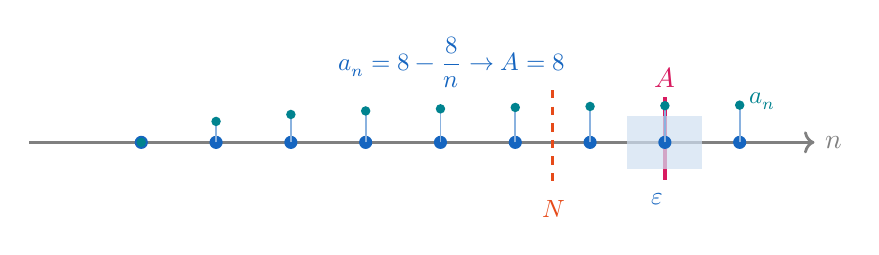
\begin{tikzpicture}[scale=0.95]
% 数轴
\draw[->, line width=1pt, gray] (-0.5,0) -- (10,0) node[right]{$n$};
% 目标值 A（数列 a_n = 8 - 8/n，极限 A=8）
\draw[cPink, line width=1.6pt] (8,0.6) -- (8,-0.5);
\node[cPink, above, font=\bfseries] at (8,0.6) {$A$};
% 误差带 epsilon（A±ε，取 ε=0.5）
\fill[cBlue!20, opacity=0.7] (7.5,-0.35) rectangle (8.5,0.35);
\node[cBlue, below, font=\small] at (8,-0.55) {$\varepsilon$ 带};
% 数列点：a_n = 8 - 8/n，取 n=1..9
% a_1=0, a_2=4, a_3=5.33, a_4=6, a_5=6.4, a_6=6.67, a_7=6.86, a_8=7, a_9=7.11
% 在图上用数列值作为 x 坐标，y 方向画出竖线表示“逼近 A”
\foreach \n/\val in {1/0, 2/4, 3/5.33, 4/6, 5/6.4, 6/6.67, 7/6.86, 8/7, 9/7.11} {
  \fill[cBlue] (\n,0) circle (2.5pt);
  \draw[cBlue!50, line width=0.7pt] (\n,0) -- (\n, {0.07*\val});
  \fill[cTeal] (\n, {0.07*\val}) circle (1.8pt);
}
\node[cTeal, right, font=\small] at (9, 0.55) {$a_n$};
\node[cBlue, above, font=\small] at (5, 0.6) {数列 $a_n=8-\dfrac{8}{n}\to A=8$};
% N 标记：n≥7 后所有点都在 ε 带内
\draw[cOrange, dashed, line width=1pt] (6.5,0.7) -- (6.5,-0.6);
\node[cOrange, below, font=\bfseries\small] at (6.5,-0.65) {$N$};
\node[cOrange, above right, font=\small] at (6.5,0.7) {之后全在带内};
\end{tikzpicture}\\[3pt]
{\small\color{gray}图 1.1\quad 数列 $\{a_n\}$ 逼近极限 $A$：越过 $N$ 后，所有点都落入 $\varepsilon$ 误差带}
\end{center}

\begin{eggbox}[冷知识：芝诺悖论与极限]
古希腊的芝诺提过一个“阿基里斯追乌龟”悖论：阿基里斯（跑得快）追乌龟（跑得慢），但要先到乌龟起点，这时乌龟爬了一段；再到那一段，乌龟又爬了……\textbf{似乎永远追不上}。这其实就是极限思想萌芽前的困惑。今天我们知道：无限段距离的\textbf{和}可以是有限的——这正是\keyw{级数}的威力。芝诺要是学了极限，就不会被乌龟难住了。
\end{eggbox}

\newpage
\subsection{函数的极限 —— 让 $x$ 去“敲门”}

数列是离散的（$n=1,2,3,\dots$），函数是连续的（$x$ 可以是任意实数）。函数极限问的是：当 $x$ 无限靠近某个值 $x_0$ 时，$f(x)$ 趋向于谁？与数列极限不同，函数极限多了一个\textbf{方向}问题：$x$ 可以从左侧（$x\to x_0^-$）或右侧（$x\to x_0^+$）分别靠近 $x_0$。当且仅当左右极限都存在且相等时，我们才说函数在 $x_0$ 处有极限。这一概念是后续讨论连续性和可导性的直接基础。

\begin{defbox}[函数极限的 $\varepsilon$–$\delta$ 定义]
设 $f$ 在 $x_0$ 的某去心邻域有定义。若 $\forall\,\varepsilon>0,\ \exists\,\delta>0$，当 $0<|x-x_0|<\delta$ 时 $|f(x)-A|<\varepsilon$，则称 $f(x)\to A\ (x\to x_0)$，记 $\displaystyle\lim_{x\to x_0}f(x)=A$。
\end{defbox}

\begin{plainbox}[白话解读：$\varepsilon$–$\delta$ 的“翻译”]
你给一个输出精度 $\varepsilon$，我就能找到一个输入范围 $\delta$——只要 $x$ 离 $x_0$ 足够近（小于 $\delta$），输出 $f(x)$ 就离 $A$ 足够近（小于 $\varepsilon$）。

注意那个 \keyw{去心}（$0<|x-x_0|$）：$x$ 可以无限靠近 $x_0$，但\textbf{不等于} $x_0$。也就是说，$f(x_0)$ 本身是什么、甚至有没有定义，都\textbf{不影响}极限。这就像“远观美人”——不一定要凑到跟前看清楚。
\end{plainbox}

\begin{thmbox}[两个重要极限 —— 必背！]
\begin{eqbox}\begin{align}
  &\lim_{x\to 0}\frac{\sin x}{x}=1, \tag{I}\\[4pt]
  &\lim_{x\to\infty}\left(1+\frac{1}{x}\right)^{x}=e. \tag{II}
\end{align}\end{eqbox}
这两个极限是求一大批极限的“母版”，务必记牢。
\end{thmbox}

\begin{quotebox}
自然这部大书是用数学语言写成的。
\qattr{伽利略（Galileo Galilei，1564--1642）}
\end{quotebox}

\begin{plainbox}[白话解读：两个重要极限长啥样？]
\begin{itemize}[leftmargin=1.4em,itemsep=3pt]
  \item 第一个（I）：\hl{$\tfrac{0}{0}$ 型}，长得像“$\tfrac{\sin(\text{小})}{\text{小}}$”，结果是 $1$。口诀：“\textbf{sin 除以自己，得 1}”。
  \item 第二个（II）：\hl{$1^{\infty}$ 型}，长得像“$(1+\text{小})^{\text{大}}$”，结果是 $e$。口诀：“\textbf{1 加上倒数，自己乘自己，得 e}”。
\end{itemize}
考试遇到这两种“长相”的极限，往这两个母版上凑就对了。
\end{plainbox}

\begin{egbox}[重要极限的应用]
求 $\displaystyle\lim_{x\to 0}\frac{1-\cos x}{x^2}$。

\textbf{解}\quad 这是 $\tfrac{0}{0}$ 型。利用 $1-\cos x=2\sin^2\!\dfrac{x}{2}$，往第一个重要极限上凑：
\begin{eqbox}\[ \lim_{x\to 0}\frac{1-\cos x}{x^2}=\lim_{x\to 0}\frac{2\sin^2(x/2)}{x^2}
   =2\left(\lim_{x\to 0}\frac{\sin(x/2)}{x}\right)^{\!2}
   =2\cdot\left(\frac{1}{2}\right)^{\!2}=\boxed{\frac{1}{2}}. \]\end{eqbox}
这里的关键技巧：把 $x^2$ 拆成 $(x/2)^2\times 4$，凑出 $\dfrac{\sin(x/2)}{x/2}$ 的结构。
\end{egbox}

\begin{warnbox}[易错警示：等价无穷小替换的“禁区”]
\begin{pkdot}
  \item \textbf{只能在乘除法中替换}，加减法中\keyw{不能}随意替换！这是最常踩的坑。
  \item \textbf{反面教材}：$\displaystyle\lim_{x\to 0}\frac{\tan x-\sin x}{x^3}$，若把 $\tan x,\sin x$ 都替换为 $x$，会得到 $\dfrac{x-x}{x^3}=0$——\textbf{大错特错}。
  \item \textbf{正确做法}：提取公因式，$\tan x-\sin x=\tan x(1-\cos x)\sim x\cdot\dfrac{x^2}{2}=\dfrac{x^3}{2}$，故极限为 $\dfrac{1}{2}$。
\end{pkdot}
\end{warnbox}

\begin{plainbox}[为什么加减法不能换？]
等价无穷小替换只保证\textbf{一阶精度}一致。加减法时，一阶项可能抵消，剩下的“差”被高阶项决定——这时还用一阶近似，就等于\keyw{把真正起作用的部分扔掉了}。所以记住：\textbf{乘除放心换，加减要小心}。
\end{plainbox}

\begin{tipbox}[常用等价无穷小速查表（$x\to 0$）]
\[
\renewcommand{\arraystretch}{1.5}
\begin{array}{ll}
\sin x\sim x & \tan x\sim x \\
\arcsin x\sim x & \arctan x\sim x \\
1-\cos x\sim \tfrac{x^2}{2} & \ln(1+x)\sim x \\
e^x-1\sim x & (1+x)^{\alpha}-1\sim \alpha x \\
\end{array}
\]
\textbf{记忆窍门}：大多数“函数在 0 附近”都等价于“$x$ 自己或 $x$ 的某次幂”——因为泰勒展开一阶项就是这个。
\end{tipbox}

\newpage
\subsection{函数的连续性 —— “不断开”的函数}

\begin{defbox}[连续的三种等价定义]
$f$ 在 $x_0$ 连续，等价于下列任一表述：
\begin{cndot}
  \item 极限式：$\displaystyle\lim_{x\to x_0}f(x)=f(x_0)$（极限值 = 函数值）
  \item 增量式：$\displaystyle\lim_{\Delta x\to 0}\Delta y=0$（自变量微变 → 因变量也微变）
  \item $\varepsilon$–$\delta$ 式：$\forall\varepsilon>0,\exists\delta>0$，$|x-x_0|<\delta\Rightarrow|f(x)-f(x_0)|<\varepsilon$
\end{cndot}
\end{defbox}

\begin{plainbox}[白话解读：连续 = “一笔画”]
连续的函数图像可以\keyw{一笔画完不断开}。不连续的点叫“间断点”，就是图像上\textbf{断开或跳跃}的地方。生活中“水温随时间变化”是连续的，“开关灯”就是不连续的（瞬间从 0 跳到 1）。
\end{plainbox}

\begin{thmbox}[闭区间上连续函数的三大定理]
\begin{cndot}
  \item \textbf{最值定理}：闭区间 $[a,b]$ 上的连续函数\textbf{必有}最大值和最小值。
  \item \textbf{有界性定理}：闭区间上的连续函数\textbf{必有界}。
  \item \textbf{介值定理}：若 $f(a)\ne f(b)$，则对 $f(a),f(b)$ 之间任一值 $\mu$，$\exists\,\xi\in(a,b)$ 使 $f(\xi)=\mu$。
\end{cndot}
\end{thmbox}

\begin{plainbox}[白话解读：三大定理的“生活版”]
\begin{itemize}[leftmargin=1.4em,itemsep=3pt]
  \item \textbf{最值定理}：一天的温度（连续变化）一定有最高点和最低点——不会“无限高”。
  \item \textbf{介值定理}：早上 8 点气温 $20°$，中午 12 点 $30°$，那么中间\textbf{一定有某个时刻}是 $25°$——温度不会“跳过”25。
  \item \textbf{注意前提}：必须是\keyw{闭区间 + 连续}。开区间或间断函数，定理可能失效。
\end{itemize}
\end{plainbox}

\begin{eggbox}[冷知识：介值定理的“急救应用”]
介值定理有个神奇推论：\textbf{把一张地图平铺在桌上，一定有一个点正好对应它正下方地表的实际位置}（不动点定理的特例）。更接地气的例子：你揉皱一张纸放到原纸上，至少有一个点没“移位”——这就是\keyw{布劳威尔不动点定理}的直观体现，介值定理是它的雏形。
\end{eggbox}

% 函数图像示意
\begin{center}
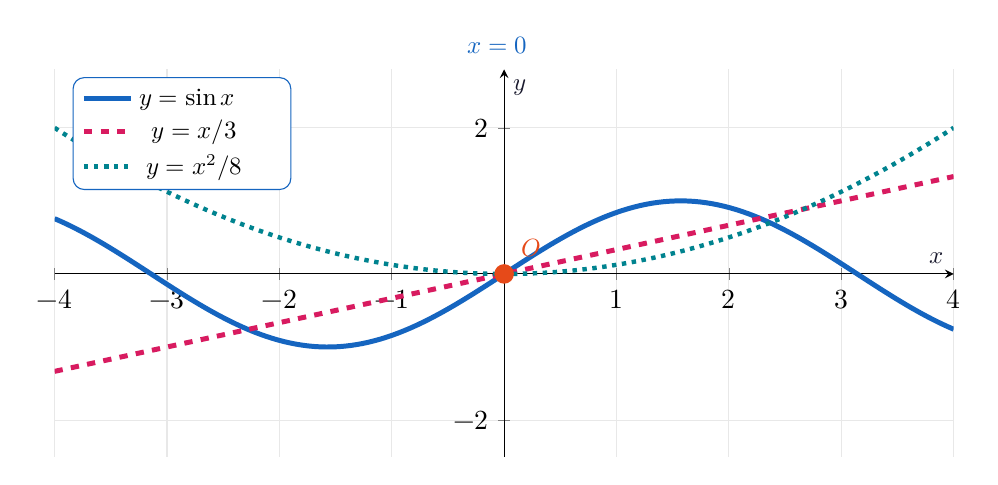
\begin{tikzpicture}
\begin{axis}[
  width=13cm, height=6.5cm,
  axis lines=middle,
  xlabel={$x$}, ylabel={$y$},
  xmin=-4, xmax=4, ymin=-2.5, ymax=2.8,
  samples=150, domain=-4:4,
  legend style={at={(0.02,0.98)}, anchor=north west, draw=cBlue, fill=white, rounded corners=4pt, font=\small},
  grid=both, grid style={gray!18},
  every axis label/.style={font=\small\color{cInk}},
  title={\small\sffamily\color{cBlue}三个函数在 $x=0$ 附近的局部行为},
  title style={yshift=-4pt}
]
\addplot[cBlue, line width=1.8pt] {sin(deg(x))};
\addlegendentry{$y=\sin x$（处处连续）}
\addplot[cPink, line width=1.8pt, dashed] {x/3};
\addlegendentry{$y=x/3$（线性）}
\addplot[cTeal, line width=1.6pt, dotted] {x*x/8};
\addlegendentry{$y=x^2/8$（抛物）}
% 标注原点
\node[circle, fill=cOrange, inner sep=2.5pt, label={above right:\small\color{cOrange}$O$}] at (axis cs:0,0) {};
\end{axis}
\end{tikzpicture}\\[3pt]
{\small\color{gray}图 1.2\quad 三类典型函数在 $x=0$ 处的局部行为比较：都连续，但“长得不一样”}
\end{center}

\begin{warnbox}[易错：连续 $\ne$ 可导]
连续只要求“不断开”，可导还要求“光滑”。经典反例：$y=|x|$ 在 $x=0$ \textbf{连续}（图像没断），但\textbf{不可导}（有个尖角，左右斜率不一样）。
\begin{eqbox}\[ \text{可导}\Rightarrow\text{连续},\quad \text{连续}\not\Rightarrow\text{可导}. \]\end{eqbox}
记住这个“单向箭头”，考试常考。
\end{warnbox}

连续与可导的关系，是分析学中最基本的“层级”关系之一。它告诉我们：\textbf{光滑比连续要求更高}。这个思想在后续学习中会不断出现——可导比连续强，二阶可导比一阶可导强，光滑函数比任意阶可导还要强。数学的假设越强，结论就越精确。

\begin{sumbox}[第一章小结 · 极限与连续]
\begin{cndot}
  \item \textbf{三大工具}：$\varepsilon$–$N$ / $\varepsilon$–$\delta$ 定义（严谨）、夹逼准则（实用）、单调有界准则（理论）。
  \item \textbf{求极限的招式}：等价无穷小（乘除法）、两个重要极限（母版）、洛必达法则（第二章）、泰勒展开（高阶）。
  \item \textbf{连续}：极限值 $=$ 函数值；闭区间连续函数有“最值 + 有界 + 介值”三大礼包。
  \item \textbf{一句话}：极限是“逼近”，连续是“不断”，可导是“光滑”——\keyw{光滑 $\Rightarrow$ 不断 $\Rightarrow$ 逼近}，反向不成立。
\end{cndot}
\end{sumbox}

\newpage

% =====================================================================
% ====================== 第二章 导数与微分 ======================
% =====================================================================
\section{导数与微分 —— “变化”的度量}

\begin{leadbox}[本章导读]
如果极限是“地基”，导数就是地基上盖起的\keyw{第一层楼}。它回答了一个朴素又深刻的问题：\textbf{这一刻，变化到底有多快？}从车速到经济增长率，从斜率到加速度，导数无处不在。
\end{leadbox}

导数的概念可以追溯到17世纪。费马在求函数极值时，已经隐约触碰到了“切线”的思想；牛顿的流数术直接将导数用于描述运动学——位置对时间的“流数”就是速度。而今天我们使用的 $f'(x)$ 记号，是拉格朗日在18世纪引入的，比牛顿的“点号”更为通用。莱布尼茨的 $\dfrac{dy}{dx}$ 记号则突出了导数作为“商”的结构，在链式法则中尤为直观。

\subsection{导数的定义 —— 从“平均”到“瞬时”}

\begin{defbox}[导数定义]
设 $y=f(x)$ 在 $x_0$ 的某邻域有定义。若极限
\begin{eqbox}\[ f'(x_0)=\lim_{\Delta x\to 0}\frac{f(x_0+\Delta x)-f(x_0)}{\Delta x}
   =\lim_{x\to x_0}\frac{f(x)-f(x_0)}{x-x_0} \]\end{eqbox}
存在，则称 $f$ 在 $x_0$ 可导，$f'(x_0)$ 为其导数。
\end{defbox}

\begin{plainbox}[白话解读：导数 = “瞬时变化率”]
那个分式 $\dfrac{f(x_0+\Delta x)-f(x_0)}{\Delta x}$ 就是\textbf{平均变化率}——在 $[x_0,x_0+\Delta x]$ 这段里，$y$ 平均每个单位 $x$ 变化多少。让 $\Delta x\to 0$，“平均”就变成“瞬时”。

生活例子：\keyw{车速}。你 2 小时开了 200 公里，平均速度 100 km/h；但某一瞬间仪表盘显示 120 km/h——那个“瞬时速度”就是\textbf{位置函数的导数}。
\end{plainbox}

\begin{warnbox}[易错：可导与连续的关系]
\textbf{可导 $\Rightarrow$ 连续，但连续 $\not\Rightarrow$ 可导。}这是高频考点。

典型反例：$y=|x|$ 在 $x=0$ 连续但不可导——左导数 $=-1$，右导数 $=1$，\keyw{左右不相等}，就像一个尖顶屋顶，左右坡度不同，顶点处“折”了一下。
\end{warnbox}

% 导数几何意义示意图
\begin{center}
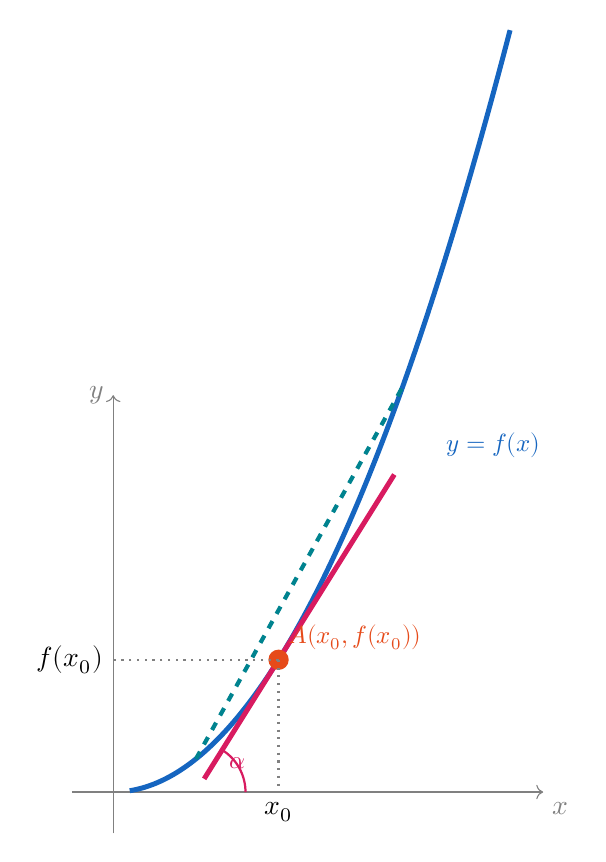
\begin{tikzpicture}[scale=1.05]
% 坐标轴
\draw[->, gray] (-0.5,0) -- (5.2,0) node[below right]{$x$};
\draw[->, gray] (0,-0.5) -- (0,4.8) node[left]{$y$};
% 曲线 y = 0.4 x^2
\draw[cBlue, line width=1.8pt, smooth, samples=100, domain=0.2:4.8]
  plot (\x, {0.4*\x*\x});
\node[cBlue, font=\small\bfseries] at (4.6,4.2) {$y=f(x)$};
% 切线: y=1.6x-1.6，从(1.1,0.16)到(3.4,3.84)
\draw[cPink, line width=1.8pt] (1.1,0.16) -- (3.4,3.84);
\node[cPink, font=\small\bfseries] at (3.6,3.7) {切线};
% 割线: 连接曲线上 (1,0.4) 和 (3.5,4.9)，斜率=1.8
\draw[cTeal, line width=1.5pt, dashed] (1,0.4) -- (3.5,4.9);
\node[cTeal, font=\small\bfseries] at (3.8,4.3) {割线};
% 切点 (2, 1.6)
\fill[cOrange] (2,1.6) circle (3.5pt);
\node[above right, cOrange, font=\small] at (2,1.6) {$A(x_0, f(x_0))$};
% 投影线
\draw[gray, dotted, line width=0.8pt] (2,1.6) -- (2,0) node[below, black]{$x_0$};
\draw[gray, dotted, line width=0.8pt] (2,1.6) -- (0,1.6) node[left, black]{$f(x_0)$};
% 角度标注：切线与 x 轴夹角 α（arctan(1.6)≈58°）
% 切线在 x=1 处过 x 轴，圆心设在 (1,0)
\draw[cPink, line width=0.8pt] (1.6,0) arc[start angle=0, end angle=58, radius=0.6];
\node[cPink, font=\small] at (1.5,0.35) {$\alpha$};
\end{tikzpicture}\\[3pt]
{\small\color{gray}图 2.1\quad 导数的几何意义：切线斜率 $\tan\alpha=f'(x_0)$；割线取极限即得切线}
\end{center}

\begin{plainbox}[白话解读：割线 → 切线]
让割线的两个端点\textbf{无限靠近}，割线就“滑动”成了切线。这个“滑动取极限”的过程，就是导数的几何本质——\keyw{切线的斜率}。所以求导数，就是在某点给函数图像“贴一条最贴合的直线”。
\end{plainbox}

\newpage
\subsection{求导法则与公式 —— “工具箱”}

\begin{tipbox}[四则运算法则 —— 求导三件套之一]
\begin{eqbox}\begin{align*}
(u\pm v)' &= u'\pm v', & &\text{（加减：各导各）} \\
(uv)' &= u'v+uv', & &\text{（乘法：交叉相乘）} \\
\left(\frac{u}{v}\right)' &= \frac{u'v-uv'}{v^2},\ v\ne 0. & &\text{（除法：上交叉下方平方）}
\end{align*}\end{eqbox}
\textbf{链式法则}（复合函数）：$\big[f(g(x))\big]'=f'(g(x))\cdot g'(x)$——\keyw{由外向内，逐层求导相乘}。
\end{tipbox}

\begin{plainbox}[白话解读：链式法则 = “剥洋葱”]
复合函数像洋葱，一层套一层。求导时从\textbf{最外层}开始，每剥一层求一次导，把各层导数\textbf{乘起来}。比如 $\sin(x^2)$：外层是 $\sin(\cdot)$，内层是 $x^2$，导数 $=\cos(x^2)\cdot 2x$。
\end{plainbox}

\begin{thmbox}[基本初等函数求导公式表 —— 必背！]
\[
\renewcommand{\arraystretch}{1.6}
\begin{array}{ll|ll}
\hline
\multicolumn{4}{l}{\textbf{常数与幂函数}} \\ \hline
(C)'=0 & (x^{\mu})'=\mu x^{\mu-1} & & \\ \hline
\multicolumn{4}{l}{\textbf{指数与对数}} \\ \hline
(a^x)'=a^x\ln a & (\log_a x)'=\dfrac{1}{x\ln a} & (e^x)'=e^x & (\ln x)'=\dfrac{1}{x} \\ \hline
\multicolumn{4}{l}{\textbf{三角函数}} \\ \hline
(\sin x)'=\cos x & (\cos x)'=-\sin x & (\tan x)'=\sec^2 x & (\cot x)'=-\csc^2 x \\ \hline
(\sec x)'=\sec x\tan x & (\csc x)'=-\csc x\cot x & & \\ \hline
\end{array}
\]
\end{thmbox}

\begin{tipbox}[记忆小窍门]
\begin{orngdot}
  \item \textbf{三角函数}：$\sin$ 和 $\cos$ 配对，$\tan$ 和 $\cot$ 配对，$\sec$ 和 $\csc$ 配对；\keyw{正号为正、余号为负}（$\sin,\tan,\sec$ 求导带正号，$\cos,\cot,\csc$ 带负号）。
  \item \textbf{指数对数}：$e^x$ 求导还是 $e^x$（“不变函数”）；$\ln x$ 求导是 $\tfrac{1}{x}$（简洁到感人）。
  \item \textbf{幂函数}：指数下来当系数，指数减一。
\end{orngdot}
\end{tipbox}

\newpage
\subsection{高阶导数与中值定理 —— “变化的变化”}

\begin{defbox}[高阶导数]
$f^{(n)}(x)=\dfrac{d^n y}{dx^n}=\big[f^{(n-1)}(x)\big]'$，即对 $f$ 连续求 $n$ 次导。

经典结论：$(\sin x)^{(n)}=\sin\!\left(x+\dfrac{n\pi}{2}\right)$，$(\cos x)^{(n)}=\cos\!\left(x+\dfrac{n\pi}{2}\right)$。
\end{defbox}

\begin{plainbox}[白话解读：高阶导数 = “套娃”]
一阶导数是“变化率”，二阶导数是“变化率的变化率”——也就是\textbf{加速度}。位置求导得速度，速度求导得加速度，加速度求导得“加加速度”（过山车的“jerky”感）……一直套娃下去。

\keyw{$\sin x$ 的高阶导数}在 $\sin$ 和 $\cos$ 之间循环：$\sin\to\cos\to-\sin\to-\cos\to\sin\to\cdots$，每求四次回到原点。那个 $\dfrac{n\pi}{2}$ 就是把这个“循环”用一个公式打包。
\end{plainbox}

\begin{thmbox}[三大中值定理 —— 沟通“函数”与“导数”的桥梁]
\begin{cndot}
  \item \textbf{罗尔定理}：$f\in C[a,b]\cap D(a,b)$，$f(a)=f(b)$ $\Rightarrow$ $\exists\,\xi\in(a,b),\ f'(\xi)=0$。
  \item \textbf{拉格朗日定理}：$f\in C[a,b]\cap D(a,b)$ $\Rightarrow$ $\exists\,\xi\in(a,b)$，$f'(\xi)=\dfrac{f(b)-f(a)}{b-a}$。
  \item \textbf{柯西定理}：$f,g\in C[a,b]\cap D(a,b)$，$g'(x)\ne 0$ $\Rightarrow$ $\exists\,\xi$，$\dfrac{f'(\xi)}{g'(\xi)}=\dfrac{f(b)-f(a)}{g(b)-g(a)}$。
\end{cndot}
\end{thmbox}

\begin{quotebox}
只要代数和几何各自分开发展，它们的进步就必然缓慢；而当它们携手合作时，便会互相促进。
\qattr{拉格朗日（Joseph-Louis Lagrange，1736--1813）}
\end{quotebox}

\begin{plainbox}[白话解读：三大定理的“旅行版”]
\begin{itemize}[leftmargin=1.4em,itemsep=3pt]
  \item \textbf{罗尔}：去程和回程高度一样，途中\textbf{至少有一刻速度为零}（水平切线）——就像爬山到顶再下来，顶点那一刻速度为 0。
  \item \textbf{拉格朗日}：从 $a$ 到 $b$，平均速度 $\dfrac{f(b)-f(a)}{b-a}$，途中\textbf{至少有一刻的瞬时速度等于平均速度}——就像“全程平均 100，某一瞬间仪表盘一定是 100”。
  \item \textbf{柯西}：拉格朗日的“双人版”——两个函数同时走，用它们的比值说话。
\end{itemize}
\end{plainbox}

\begin{center}
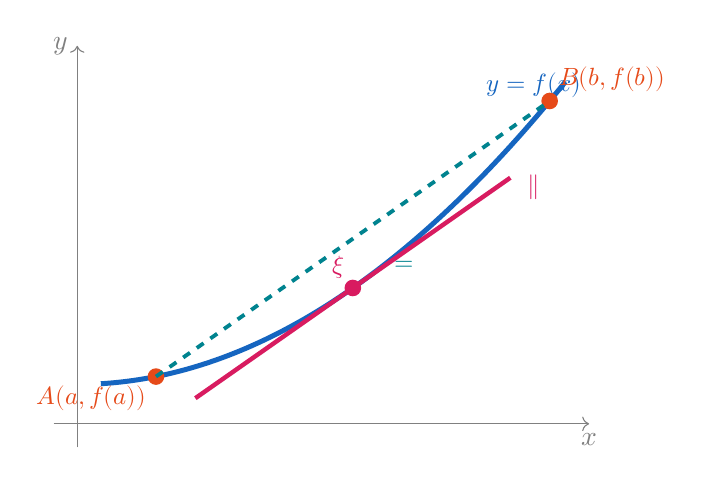
\begin{tikzpicture}[scale=1.0]
% 坐标轴
\draw[->, gray] (-0.3,0) -- (6.5,0) node[below]{$x$};
\draw[->, gray] (0,-0.3) -- (0,4.8) node[left]{$y$};
% 曲线 f(x)=0.1x^2+0.5
\draw[cBlue, line width=1.8pt, smooth, samples=120, domain=0.3:6.2]
  plot (\x, {0.1*\x*\x+0.5});
\node[cBlue, font=\small\bfseries] at (5.8,4.3) {$y=f(x)$};
% 端点 A=(1,0.6), B=(6,4.1)
\fill[cOrange] (1,0.6) circle (3pt);
\node[below left, cOrange, font=\small] at (1,0.6) {$A(a,f(a))$};
\fill[cOrange] (6,4.1) circle (3pt);
\node[above right, cOrange, font=\small] at (6,4.1) {$B(b,f(b))$};
% 割线 AB: 斜率=0.7, y=0.7x-0.1
\draw[cTeal, line width=1.4pt, dashed] (1,0.6) -- (6,4.1);
\node[cTeal, font=\small] at (4.2,2.0) {割线（斜率$=$平均变化率）};
% 切线在 ξ=3.5 处, f(ξ)=1.725, 切线: y=0.7x-0.725
% 从(1.5,0.325)到(5.5,3.125)
\fill[cPink] (3.5,1.725) circle (3pt);
\node[above left, cPink, font=\small] at (3.5,1.725) {$\xi$};
\draw[cPink, line width=1.6pt] (1.5,0.325) -- (5.5,3.125);
\node[cPink, font=\small] at (5.8,3.0) {切线（$\parallel$割线）};
\end{tikzpicture}\\[3pt]
{\small\color{gray}图 2.2\quad 拉格朗日定理的几何意义：$\exists\,\xi$，切线 $\parallel$ 割线 $AB$}
\end{center}

\begin{egbox}[验证拉格朗日定理]
验证 $f(x)=x^3$ 在 $[0,1]$ 上满足拉格朗日定理并求 $\xi$。

\textbf{解}\quad $f\in C[0,1]\cap D(0,1)$（多项式处处连续可导，条件满足）。
平均变化率：$\dfrac{f(1)-f(0)}{1-0}=\dfrac{1-0}{1}=1$。
令 $f'(\xi)=3\xi^2=1$，解得 $\xi=\dfrac{1}{\sqrt{3}}=\dfrac{\sqrt{3}}{3}\in(0,1)$。$\boxed{\xi=\frac{\sqrt{3}}{3}}$
\end{egbox}

\newpage
\subsection{洛必达法则 —— 不定式的“救星”}

\begin{thmbox}[洛必达法则（$\tfrac{0}{0}$ 或 $\tfrac{\infty}{\infty}$ 型）]
若 $\displaystyle\lim_{x\to a}\frac{f(x)}{g(x)}$ 为 $\tfrac{0}{0}$ 或 $\tfrac{\infty}{\infty}$ 型，且 $f,g$ 在 $a$ 的去心邻域可导、$g'\ne 0$，若 $\displaystyle\lim_{x\to a}\frac{f'(x)}{g'(x)}=A$（或 $\infty$），则
\begin{eqbox}\[ \lim_{x\to a}\frac{f(x)}{g(x)}=A\ (\text{或}\ \infty). \]\end{eqbox}
\end{thmbox}

\begin{plainbox}[白话解读：洛必达 = “上下同时求导”]
遇到 $\tfrac{0}{0}$ 或 $\tfrac{\infty}{\infty}$ 这种“算不出”的分式，\keyw{分子分母同时求导}再试。原理是：当 $f,g$ 都趋于 $0$（或 $\infty$）时，它们的“\textbf{变化速度之比}”决定了“\textbf{最终值之比}”。

口诀：\keyw{“零比零、无穷比无穷，上下求导接着算”}。
\end{plainbox}

\begin{egbox}[洛必达法则求极限]
求 $\displaystyle\lim_{x\to 0}\frac{x-\sin x}{x^3}$。

\textbf{解}\quad 这是 $\tfrac{0}{0}$ 型，连续使用洛必达（每次用前都要验证型别）：
\begin{eqbox}\[ \lim_{x\to 0}\frac{x-\sin x}{x^3}
   \overset{L}{=}\lim_{x\to 0}\frac{1-\cos x}{3x^2}
   \overset{L}{=}\lim_{x\to 0}\frac{\sin x}{6x}
   =\boxed{\frac{1}{6}}. \]\end{eqbox}
最后一步用了重要极限 $\dfrac{\sin x}{x}\to 1$。注意：洛必达用了两次，每次都是 $\tfrac{0}{0}$ 型，符合使用条件。
\end{egbox}

\begin{warnbox}[易错：洛必达的三大误用]
\begin{pkdot}
  \item \textbf{不验证型别就用}：必须先确认是 $\tfrac{0}{0}$ 或 $\tfrac{\infty}{\infty}$，否则会出错。
  \item \textbf{导数比不存在就下结论}：若 $\lim\dfrac{f'}{g'}$ \textbf{不存在也非无穷}，\keyw{不能}断言原极限不存在——法则只是“失效”，换个方法可能还能算。
  \item \textbf{滥用洛必达}：能用等价无穷小的，优先用等价无穷小，往往更简洁。洛必达是“最后手段”，不是“第一反应”。
\end{pkdot}
\end{warnbox}

\begin{eggbox}[冷知识：洛必达法则其实是“买来的”]
洛必达侯爵是个贵族数学爱好者，他\textbf{花钱雇}了瑞士数学家约翰·伯努利来讲课，并在合同里约定：伯努利的数学发现可以归洛必达使用。于是伯努利发明的这个法则，被洛必达写进自己的教材《无穷小分析》里，署了洛必达的名字——\keyw{史上最著名的“代笔”}之一。直到洛必达去世后，伯努利才“维权”成功。所以严谨地说，这该叫“伯努利法则”。
\end{eggbox}

% 速度-时间-加速度关系图
\begin{center}
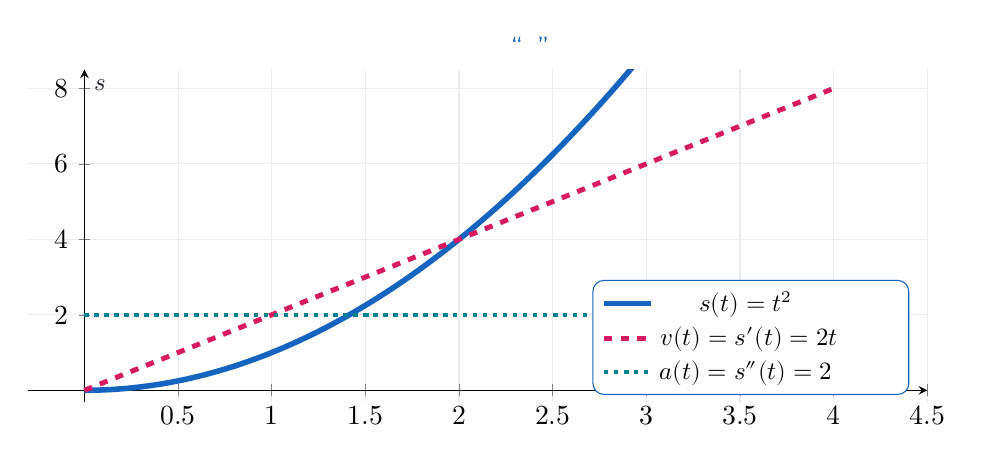
\begin{tikzpicture}
\begin{axis}[
  width=13cm, height=5.8cm,
  axis lines=middle,
  xlabel={$t$（时间）}, ylabel={$s$（位置）},
  xmin=-0.3, xmax=4.5, ymin=-0.3, ymax=8.5,
  samples=120, domain=0:4,
  legend style={at={(0.98,0.02)}, anchor=south east, draw=cBlue, fill=white, rounded corners=4pt, font=\small},
  grid=both, grid style={gray!15},
  every axis label/.style={font=\small\color{cInk}},
  title={\small\sffamily\color{cBlue}位置、速度、加速度：高阶导数的“套娃”},
  title style={yshift=-4pt}
]
% 位置 s = t^2
\addplot[cBlue, line width=2pt] {x*x};
\addlegendentry{$s(t)=t^2$（位置，二阶可导）}
% 速度 v = 2t
\addplot[cPink, line width=1.8pt, dashed] {2*x};
\addlegendentry{$v(t)=s'(t)=2t$（速度，一阶导）}
% 加速度 a = 2
\addplot[cTeal, line width=1.6pt, dotted] {2};
\addlegendentry{$a(t)=s''(t)=2$（加速度，二阶导）}
\end{axis}
\end{tikzpicture}\\[3pt]
{\small\color{gray}图 2.3\quad 导数的“套娃”：位置求导得速度，再求导得加速度}
\end{center}

\begin{sumbox}[第二章小结 · 导数与微分]
\begin{cndot}
  \item \textbf{导数} = 瞬时变化率 = 切线斜率；\keyw{可导 $\Rightarrow$ 连续}，反之不然。
  \item \textbf{求导三件套}：公式表（背）、四则法则（加减乘除）、链式法则（剥洋葱）。
  \item \textbf{中值定理}：连接“函数值”与“导数值”的桥梁，是证明题的核心工具——罗尔是拉格朗日的特例，拉格朗日是柯西的特例。
  \item \textbf{洛必达法则}：不定式 $\tfrac{0}{0},\tfrac{\infty}{\infty}$ 的利器，但\keyw{先验证、防滥用}，能用等价无穷小就优先用。
  \item \textbf{一句话}：导数把“变化”变成了一个可计算的数，从此“快慢”有了刻度。
\end{cndot}
\end{sumbox}

\newpage

% =====================================================================
% ====================== 第三章 不定积分 ======================
% =====================================================================
\section{不定积分 —— “逆向”的智慧}

\begin{leadbox}[本章导读]
积分是导数的\keyw{逆运算}。求导是“顺水推舟”，积分是“逆水行舟”——所以积分\textbf{比求导难}。但别怕，掌握方法后你会发现，它有种“拼图还原”的乐趣。
\end{leadbox}

积分的思想比导数更古老。阿基米德在公元前3世纪就用“穷竭法”计算了抛物线弓形的面积——这可以看作积分的雏形。但真正的突破要等到17世纪，牛顿和莱布尼茨各自发现了“微积分基本定理”，揭示了积分与导数之间的深刻联系：\textbf{积分是导数的逆运算}。从此，求面积、求体积、求弧长这些看似各不相同的问题，统一到了一个框架之下。而莱布尼茨发明的 $\int$ 符号——拉丁文 \textit{summa}（求和）首字母 $S$ 的拉长版——至今仍是最优美的数学符号之一。

\subsection{原函数与不定积分 —— “找回来”}

\begin{defbox}[原函数与不定积分]
若 $F'(x)=f(x)$，则称 $F$ 为 $f$ 的一个\textbf{原函数}。若 $f$ 有原函数，则其全体原函数为 $F(x)+C$（$C$ 为任意常数），记作
\begin{eqbox}\[ \int f(x)\,dx = F(x)+C,\quad C\in\mathbb{R}. \]\end{eqbox}
\end{defbox}

\begin{plainbox}[白话解读：积分 = “找回原函数”]
求导是“把函数拆了”，积分是“把拆掉的东西\textbf{拼回去}”。比如知道速度 $v(t)$，想还原位置 $s(t)$——这就是积分。

那个\keyw{$+C$} 千万别忘！因为求导时常数会消失（$(F+C)'=F'=f$），所以“拼回去”时，丢失的常数\textbf{找不回来了}，只能用一个 $C$ 表示“任意常数”。考试忘写 $+C$，扣分没商量。
\end{plainbox}

\begin{tipbox}[原函数存在定理]
若 $f$ 在区间 $I$ 上\textbf{连续}，则 $f$ 在 $I$ 上\textbf{必有}原函数。

\textbf{注意}：这只是“存在性”，不保证“能算出来”。有些连续函数的原函数\keyw{写不出初等函数表达式}（比如 $e^{-x^2}$），这叫“非初等可积”。
\end{tipbox}

\begin{eggbox}[冷知识：$e^{-x^2}$ 的原函数“不存在”？]
$e^{-x^2}$ 是概率论里标准正态分布的核心函数，它的图像是个漂亮的钟形曲线。但它\textbf{没有初等函数形式的原函数}——也就是说，你无法用 $+,-,\times,\div,\sin,\cos,\ln,e^x$ 这些“常规零件”拼出一个 $\int e^{-x^2}dx$。

这不是数学家偷懒，而是\keyw{已被严格证明}的不可能。所以概率论里算正态分布概率，用的是数值方法或查表。数学也有“到此为止”的边界，这种“无解之美”反而很迷人。
\end{eggbox}

% 积分与导数关系示意
\begin{center}
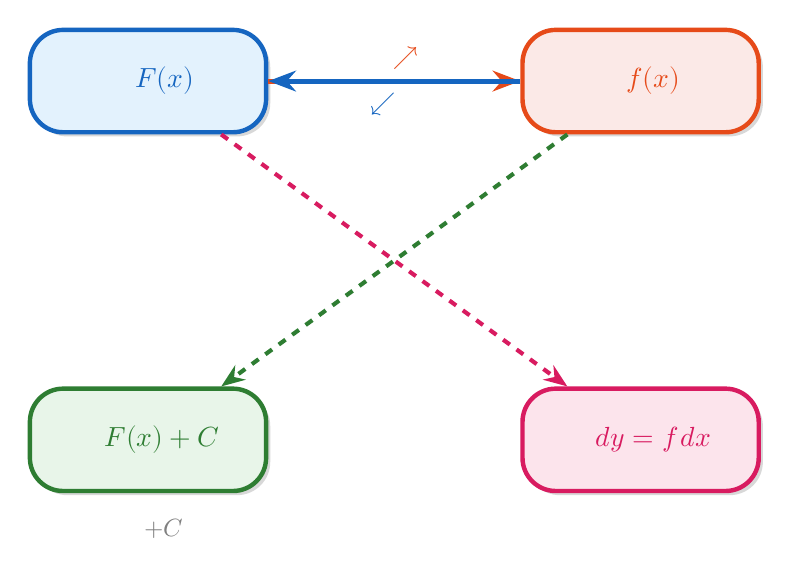
\begin{tikzpicture}[
  node distance=3.2cm,
  box/.style={draw, rounded corners=12pt, line width=1.6pt,
              minimum width=3cm, minimum height=1.3cm,
              font=\sffamily\bfseries, align=center,
              drop shadow={shadow xshift=1.5pt,shadow yshift=-1.5pt,opacity=0.3}}
]
\node[box, fill=cBlueL, draw=cBlue, text=cBlue] (f) {原函数 $F(x)$};
\node[box, fill=cOrangeL, draw=cOrange, text=cOrange, right=of f] (fp) {导数 $f(x)$};
\node[box, fill=cGreenL, draw=cGreen, text=cGreen, below=of f] (int) {积分 $F(x)+C$};
\node[box, fill=cPinkL, draw=cPink, text=cPink, below=of fp] (der) {微分 $dy=f\,dx$};

\draw[->, cOrange, line width=1.8pt, -{Stealth[length=3.5mm]}]
  (f) -- node[above, font=\small\sffamily\bfseries, text=cOrange]{求导 $\nearrow$} (fp);
\draw[->, cBlue, line width=1.8pt, -{Stealth[length=3.5mm]}]
  (fp) -- node[below, font=\small\sffamily\bfseries, text=cBlue]{$\swarrow$ 积分} (f);
\draw[->, cPink, line width=1.5pt, -{Stealth[length=3mm]}, dashed]
  (f) -- node[left, font=\small\sffamily\bfseries, text=cPink]{微分} (der);
\draw[->, cGreen, line width=1.5pt, -{Stealth[length=3mm]}, dashed]
  (fp) -- node[right, font=\small\sffamily\bfseries, text=cGreen]{不定积分} (int);
\node[font=\small\color{gray}, below=0.2cm of int] {（结果带 $+C$）};
\end{tikzpicture}\\[3pt]
{\small\color{gray}图 3.1\quad 导数与积分：互逆运算，就像“拆”与“拼”}
\end{center}

\newpage
\subsection{基本积分表 —— “逆向背诵”}

\begin{thmbox}[基本积分公式表 —— 必背！]
\[
\renewcommand{\arraystretch}{1.7}
\begin{array}{ll}
\hline
\displaystyle\int k\,dx=kx+C & \displaystyle\int x^{\mu}\,dx=\frac{x^{\mu+1}}{\mu+1}+C\ (\mu\ne -1) \\ \hline
\displaystyle\int \frac{1}{x}\,dx=\ln|x|+C & \displaystyle\int e^x\,dx=e^x+C \\ \hline
\displaystyle\int \sin x\,dx=-\cos x+C & \displaystyle\int \cos x\,dx=\sin x+C \\ \hline
\displaystyle\int \sec^2 x\,dx=\tan x+C & \displaystyle\int \csc^2 x\,dx=-\cot x+C \\ \hline
\displaystyle\int \frac{1}{1+x^2}\,dx=\arctan x+C & \displaystyle\int \frac{1}{\sqrt{1-x^2}}\,dx=\arcsin x+C \\ \hline
\end{array}
\]
\end{thmbox}

\begin{tipbox}[记忆诀窍：积分表 = 导数表“反过来”]
积分公式就是求导公式的\keyw{逆向}。把求导公式从右往左读，就是积分公式。所以\textbf{求导表背熟了，积分表免费送}——前提是你得能“逆向反应”。

两个易错点：
\begin{pkdot}
  \item $\displaystyle\int\frac{1}{x}\,dx=\ln|x|+C$，\textbf{绝对值不能漏}（$x$ 可正可负）。
  \item $\displaystyle\int\sin x\,dx=-\cos x+C$，\textbf{那个负号别忘了}。
\end{pkdot}
\end{tipbox}

\newpage
\subsection{积分方法 —— “三大法宝”}

积分比求导难，难在\textbf{没有万能算法}，要靠“识别题型 + 套方法”。下面是三大法宝。

\begin{tipbox}[法宝一：第一换元法（凑微分）]
若 $\int f(u)\,du=F(u)+C$，则
\begin{eqbox}\[ \int f\big(\varphi(x)\big)\varphi'(x)\,dx = F\big(\varphi(x)\big)+C. \]\end{eqbox}
\textbf{核心思路}：把被积式中的一部分“\keyw{凑}”成某函数的微分，再整体换元。
\end{tipbox}

\begin{plainbox}[白话解读：凑微分 = “看顺眼”]
被积函数里若有“某函数 $\times$ 它的导数”这种组合，就把导数那部分凑成微分。比如 $\dfrac{1}{x}$ 正好是 $\ln x$ 的导数，那就把 $\dfrac{dx}{x}$ 凑成 $d(\ln x)$。

口诀：\keyw{“看见导数，凑成微分；整体换元，海阔天空”}。
\end{plainbox}

\begin{egbox}[凑微分法]
求 $\displaystyle\int \frac{1}{x\ln x}\,dx$。

\textbf{解}\quad 敏锐地发现 $\dfrac{1}{x}dx=d(\ln x)$，令 $u=\ln x$：
\begin{eqbox}\[ \int \frac{1}{x\ln x}\,dx=\int \frac{1}{\ln x}\,d(\ln x)=\int \frac{du}{u}=\ln|u|+C=\boxed{\ln|\ln x|+C}. \]\end{eqbox}
这道题的“眼力”在于：把 $\ln x$ 整体看作 $u$，而 $\dfrac{1}{x}dx$ 恰好是 $du$——\keyw{天作之合}。
\end{egbox}

\begin{tipbox}[法宝二：第二换元法（三角换元）]
遇到根号，用三角恒等式消掉：
\begin{cndot}
  \item 含 $\sqrt{a^2-x^2}$：令 $x=a\sin t$（用 $1-\sin^2 t=\cos^2 t$）
  \item 含 $\sqrt{a^2+x^2}$：令 $x=a\tan t$（用 $1+\tan^2 t=\sec^2 t$）
  \item 含 $\sqrt{x^2-a^2}$：令 $x=a\sec t$（用 $\sec^2 t-1=\tan^2 t$）
\end{cndot}
\end{tipbox}

\begin{plainbox}[白话解读：三角换元 = “消根号”]
根号是积分的头号敌人。三角恒等式里藏着“平方和/差”的恒等式，正好能\textbf{把根号里的平方抵消掉}。换元后根号消失，世界清净了。

记忆：\keyw{“根号里是减号用 sin，加号用 tan，$x^2-a^2$ 用 sec”}。
\end{plainbox}

\newpage
\begin{egbox}[三角换元]
求 $\displaystyle\int \sqrt{1-x^2}\,dx$。

\textbf{解}\quad 根号里是 $1-x^2$（减号），令 $x=\sin t$（$t\in[-\tfrac{\pi}{2},\tfrac{\pi}{2}]$），$dx=\cos t\,dt$：
\begin{eqbox}\begin{align*}
\int \sqrt{1-x^2}\,dx &= \int \cos t\cdot\cos t\,dt=\int \cos^2 t\,dt\\
  &= \frac{1}{2}\int(1+\cos 2t)\,dt=\frac{t}{2}+\frac{\sin 2t}{4}+C\\
  &= \frac{1}{2}\arcsin x+\frac{1}{2}x\sqrt{1-x^2}+C.
\end{align*}\end{eqbox}
最后一步用 $t=\arcsin x$ 回代，$\sin 2t=2\sin t\cos t=2x\sqrt{1-x^2}$。
\begin{eqbox}\[ \boxed{\int \sqrt{1-x^2}\,dx=\tfrac{1}{2}\arcsin x+\tfrac{1}{2}x\sqrt{1-x^2}+C} \]\end{eqbox}
\end{egbox}

\begin{warnbox}[易错：换元的“两个别忘了”]
\begin{pkdot}
  \item \textbf{回代}：换元后结果用 $t$ 表示，必须\keyw{换回 $x$}——答案不能留 $t$。
  \item \textbf{定义域}：三角换元要限定 $t$ 的范围，确保\textbf{根号前符号正确}（通常取主值区间，保证 $\cos t,\sec t$ 为正）。
  \item \textbf{系数配平}：凑微分时 $dx=\dfrac{1}{a}d(ax+b)$，那个 $\dfrac{1}{a}$ 别丢了。
\end{pkdot}
\end{warnbox}

\begin{tipbox}[法宝三：分部积分法]
\begin{eqbox}\[ \int u\,dv=uv-\int v\,du \]\end{eqbox}
\textbf{选 $u$ 的口诀（LIATE 法则）}：优先级从左到右——
\begin{orngdot}
  \item \textbf{L}ogarithm（对数函数）
  \item \textbf{I}nverse trig（反三角函数）
  \item \textbf{A}lgebraic（代数/多项式）
  \item \textbf{T}rigonometric（三角函数）
  \item \textbf{E}xponential（指数函数）
\end{orngdot}
排前者选作 $u$（求导后变简单），排后者选作 $dv$（积分后不复杂）。
\end{tipbox}

\begin{plainbox}[白话解读：分部积分 = “转嫁矛盾”]
有些积分里两部分“扭打在一起”，谁也积不动。分部积分的套路是：把一部分\textbf{求导}（变简单），另一部分\textbf{积分}（保持可控），让原来的 $\int u\,dv$ 变成新的 $\int v\,du$——\keyw{换个位置，难题变易题}。

选 $u$ 的原则：\textbf{求导后变简单的当 $u$}。对数、反三角求导后变成代数式，“瘦身”明显，所以优先当 $u$。
\end{plainbox}

\begin{egbox}[分部积分]
求 $\displaystyle\int x e^x\,dx$。

\textbf{解}\quad 按 LIATE，$x$ 是代数（A），$e^x$ 是指数（E），选 $u=x$。
取 $u=x,\ dv=e^x dx$，则 $du=dx,\ v=e^x$：
\begin{eqbox}\[ \int x e^x\,dx = xe^x-\int e^x\,dx = xe^x-e^x+C=\boxed{e^x(x-1)+C}. \]\end{eqbox}
看，$x$ 求导变成 $1$（变简单了），$e^x$ 积分还是 $e^x$（没变复杂）——完美的“转嫁”。
\end{egbox}

% 分部积分“转嫁”示意图
\begin{center}
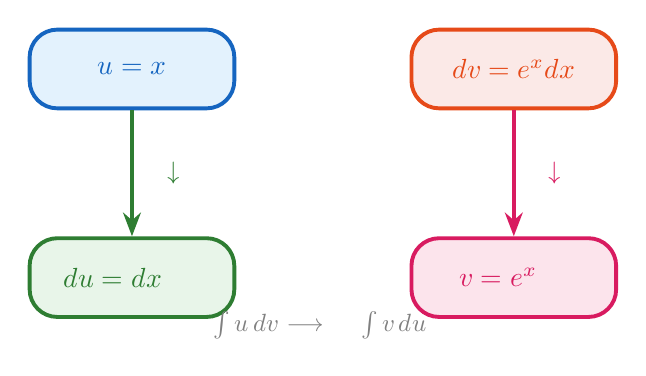
\begin{tikzpicture}[
  node distance=1.6cm,
  pill/.style={rounded corners=10pt, draw, line width=1.4pt,
               minimum width=2.6cm, minimum height=1cm,
               font=\sffamily\bfseries, align=center}
]
\node[pill, fill=cBlueL, draw=cBlue, text=cBlue] (u1) {$u=x$};
\node[pill, fill=cOrangeL, draw=cOrange, text=cOrange, right=2.2cm of u1] (v1) {$dv=e^x dx$};
\node[pill, fill=cGreenL, draw=cGreen, text=cGreen, below=of u1] (u2) {$du=dx$（变简单）};
\node[pill, fill=cPinkL, draw=cPink, text=cPink, below=of v1] (v2) {$v=e^x$（可控）};

\draw[->, cGreen, line width=1.6pt, -{Stealth[length=3mm]}]
  (u1) -- node[right, font=\small\bfseries, text=cGreen]{求导 $\downarrow$} (u2);
\draw[->, cPink, line width=1.6pt, -{Stealth[length=3mm]}]
  (v1) -- node[right, font=\small\bfseries, text=cPink]{积分 $\downarrow$} (v2);
\node[font=\small\color{gray}, below=0.3cm of $(u2)!0.5!(v2)$] {原积分 $\int u\,dv$ $\longrightarrow$ 新积分 $\int v\,du$（更简单）};
\end{tikzpicture}\\[3pt]
{\small\color{gray}图 3.2\quad 分部积分的“转嫁”：$u$ 求导变简单，$dv$ 积分保持可控}
\end{center}

\begin{eggbox}[冷知识：积分符号 $\int$ 的来历]
莱布尼茨在 1675 年发明了积分号 $\int$——它是拉丁文 \textit{summa}（求和）首字母 $S$ 的\keyw{拉长版}。因为积分本质是“无限项求和”，莱布尼茨就用一个拉长的 $S$ 来表示。而 $dx$ 表示“无穷小增量”。这套符号直观又优雅，沿用至今三百多年没变过——好符号和好数学一样，经得起时间。
\end{eggbox}

\begin{sumbox}[第三章小结 · 不定积分]
\begin{cndot}
  \item \textbf{不定积分} = 求原函数族，结果\keyw{必须加 $+C$}（高频扣分点）。
  \item \textbf{三大法宝}：凑微分（最常用，靠眼力）、换元法（三角换元消根号）、分部积分（LIATE 选 $u$）。
  \item \textbf{积分表} = 导数表的逆向，背熟求导表就送积分表。
  \item \textbf{积分比求导难}：求导有固定算法，积分靠\keyw{识别题型}——多练多记是唯一捷径。
  \item \textbf{一句话}：积分是“逆向拼图”，虽然难，但拼对的瞬间很爽。
\end{cndot}
\end{sumbox}

\newpage

% ====================== 结语页 ======================
\section*{\color{cBlue}结语 · 数学是一场马拉松}
\addcontentsline{toc}{section}{结语}

\begin{center}

\begin{tikzpicture}
\node[fill=cBlueL, draw=cBlue, line width=1.6pt, rounded corners=18pt,
      inner xsep=24pt, inner ysep=14pt, drop shadow={shadow xshift=2pt,shadow yshift=-2pt,opacity=0.35},
      text width=13.5cm, align=center]
  {\Large\sffamily\color{cBlue}\textbf{数学是自然的语言，而微积分是其中最优雅的篇章。}\\[10pt]
   \normalsize\color{cInk}这份笔记从极限走到积分，画出了微积分的骨架。\\
   但真正的血肉，要靠你\textbf{一道题一道题}地填充。\\[6pt]
   别怕犯错——每一个算错的积分，都是通往正确的路标；\\
   每一个想不通的证明，都是思维在拔节生长的声音。};
\end{tikzpicture}
\end{center}


\begin{quotebox}
数学家不是因为数学有用才研究它，而是因为数学美才乐此不疲。
\qattr{庞加莱（Henri Poincaré，1854--1912）}
\end{quotebox}

\begin{plainbox}[写给坚持到这里的你]
高数这门课，有人觉得是“拦路虎”，有人觉得是“敲门砖”。但愿你读完这份笔记后，能多看到一点它的\keyw{美}——

极限告诉我们“\textbf{无限逼近}也是一种到达”；导数告诉我们“\textbf{变化}可以被精确度量”；积分告诉我们“\textbf{积累}的力量不可小觑”。

这三句话，何尝不是人生的注脚？

\hfill ——与君共勉
\end{plainbox}

\vspace{0.8cm}

\begin{center}

\begin{tikzpicture}
\foreach \c/\x in {cBlue/0, cPink/1.2, cYellow/2.4, cTeal/3.6, cPurple/4.8, cOrange/6.0, cGreen/7.2}
  \fill[\c] (\x,0) circle (0.42);
\end{tikzpicture}\\[12pt]
{\large\sffamily\color{cBlue}\textbf{— 完 —}}
\end{center}

\vfill
\begin{center}
\small\color{gray}
编者：杨建伟 \quad|\quad 华北水利水电大学 数学与统计学院\\
本笔记采用 \LaTeX{} 排版，使用 ctex + tcolorbox + TikZ + pgfplots 制作\\
\textit{愿你在数学的世界里，走得远，也走得开心。}
\end{center}

\end{document}
